\documentclass[a4paper,11pt]{book}
%\documentclass[a4paper,twoside,11pt,titlepage]{book}
\usepackage{listings}
\usepackage[utf8]{inputenc}
\usepackage[spanish]{babel}

% \usepackage[style=list, number=none]{glossary} %
%\usepackage{titlesec}
%\usepackage{pailatino}

\decimalpoint
\usepackage{dcolumn}
\newcolumntype{.}{D{.}{\esperiod}{-1}}
\makeatletter
\addto\shorthandsspanish{\let\esperiod\es@period@code}
\makeatother


%\usepackage[chapter]{algorithm}
\RequirePackage{verbatim}
%\RequirePackage[Glenn]{fncychap}
\usepackage{fancyhdr}
\usepackage{graphicx}
\usepackage{afterpage}

\usepackage{longtable}

\usepackage[pdfborder={000}]{hyperref} %referencia

% ********************************************************************
% Re-usable information
% ********************************************************************
\newcommand{\myTitle}{TradingAPP}
\newcommand{\mySubtitle}{Aplicación web para trading algorítmico}
\newcommand{\mySubtitleEnglish}{Algorithmic trading web application}
\newcommand{\myDegree}{Grado en ingeniería informática}
\newcommand{\myName}{Manuel Carmona Pérez}
\newcommand{\myProf}{José Manuel Benítez Sánchez}
%\newcommand{\mySupervisor}{Put name here}
\newcommand{\myFaculty}{Escuela Técnica Superior de Ingenierías Informática y de
Telecomunicación}
\newcommand{\myFacultyShort}{E.T.S. de Ingenierías Informática y de
Telecomunicación}
\newcommand{\myDepartment}{Departamento de ...}
\newcommand{\myUni}{\protect{Universidad de Granada}}
\newcommand{\myLocation}{Granada}
\newcommand{\myTime}{\today}
\newcommand{\myVersion}{Version 0.1}


\hypersetup{
pdfauthor = {\myName (email (en) ugr (punto) es)},
pdftitle = {\myTitle},
pdfsubject = {},
pdfkeywords = {palabra_clave1, palabra_clave2, palabra_clave3, ...},
pdfcreator = {LaTeX con el paquete ....},
pdfproducer = {pdflatex}
}

%\hyphenation{}


%\usepackage{doxygen/doxygen}
%\usepackage{pdfpages}
\usepackage{url}
\usepackage{colortbl,longtable}
\usepackage[stable]{footmisc}
\usepackage{index}

\makeindex
%\usepackage[style=long, cols=2,border=plain,toc=true,number=none]{glossary}
% \makeglossary

% Definición de comandos que me son tiles:
%\renewcommand{\indexname}{Índice alfabético}
%\renewcommand{\glossaryname}{Glosario}

\pagestyle{fancy}
\fancyhf{}
\fancyhead[LO]{\leftmark}
\fancyhead[RE]{\rightmark}
\fancyhead[RO,LE]{\textbf{\thepage}}
\renewcommand{\chaptermark}[1]{\markboth{\textbf{#1}}{}}
\renewcommand{\sectionmark}[1]{\markright{\textbf{\thesection. #1}}}

\setlength{\headheight}{1.5\headheight}

\newcommand{\HRule}{\rule{\linewidth}{0.5mm}}
%Definimos los tipos teorema, ejemplo y definición podremos usar estos tipos
%simplemente poniendo \begin{teorema} \end{teorema} ...
\newtheorem{teorema}{Teorema}[chapter]
\newtheorem{ejemplo}{Ejemplo}[chapter]
\newtheorem{definicion}{Definición}[chapter]

\definecolor{gray97}{gray}{.97}
\definecolor{gray75}{gray}{.75}
\definecolor{gray45}{gray}{.45}
\definecolor{gray30}{gray}{.94}

\lstset{ frame=Ltb,
     framerule=0.5pt,
     aboveskip=0.5cm,
     framextopmargin=3pt,
     framexbottommargin=3pt,
     framexleftmargin=0.1cm,
     framesep=0pt,
     rulesep=.4pt,
     backgroundcolor=\color{gray97},
     rulesepcolor=\color{black},
     %
     stringstyle=\ttfamily,
     showstringspaces = false,
     basicstyle=\scriptsize\ttfamily,
     commentstyle=\color{gray45},
     keywordstyle=\bfseries,
     %
     numbers=left,
     numbersep=6pt,
     numberstyle=\tiny,
     numberfirstline = false,
     breaklines=true,
   }
 
% minimizar fragmentado de listados
\lstnewenvironment{listing}[1][]
   {\lstset{#1}\pagebreak[0]}{\pagebreak[0]}

\lstdefinestyle{CodigoC}
   {
	basicstyle=\scriptsize,
	frame=single,
	language=C,
	numbers=left
   }
\lstdefinestyle{CodigoC++}
   {
	basicstyle=\small,
	frame=single,
	backgroundcolor=\color{gray30},
	language=C++,
	numbers=left
   }

 
\lstdefinestyle{Consola}
   {basicstyle=\scriptsize\bf\ttfamily,
    backgroundcolor=\color{gray30},
    frame=single,
    numbers=none
   }


\newcommand{\bigrule}{\titlerule[0.5mm]}


%Para conseguir que en las páginas en blanco no ponga cabecerass
\makeatletter
\def\clearpage{%
  \ifvmode
    \ifnum \@dbltopnum =\m@ne
      \ifdim \pagetotal <\topskip
        \hbox{}
      \fi
    \fi
  \fi
  \newpage
  \thispagestyle{empty}
  \write\m@ne{}
  \vbox{}
  \penalty -\@Mi
}
\makeatother

\usepackage{pdfpages}
\begin{document}
\begin{titlepage}
 
 
\newlength{\centeroffset}
\setlength{\centeroffset}{-0.5\oddsidemargin}
\addtolength{\centeroffset}{0.5\evensidemargin}
\thispagestyle{empty}

\noindent\hspace*{\centeroffset}\begin{minipage}{\textwidth}

\centering

\includegraphics[width=0.9\textwidth]{imagenes/logo_ugr.jpg}\\[1.4cm]

\textsc{ \Large TRABAJO FIN DE GRADO\\[0.2cm]}
\textsc{ INGENIERÍA INFORMÁTICA }\\[1cm]
% Upper part of the page
% 
% Title
{\Huge\bfseries \myTitle \\}
\noindent\rule[-1ex]{\textwidth}{3pt}\\[3.5ex]
{\large\bfseries \mySubtitle \\}
\end{minipage}

\vspace{2.5cm}
\noindent\hspace*{\centeroffset}\begin{minipage}{\textwidth}
\centering

\textbf{Autor}\\ { \myName }\\[2.5ex]
\textbf{Director}\\
{ \myProf }\\[2cm]

\includegraphics[width=0.3\textwidth]{imagenes/etsiit_logo.png}\\[0.1cm]
\textsc{\myFaculty}\\
\textsc{---}\\
Granada, mes de 2021
\end{minipage}
%\addtolength{\textwidth}{\centeroffset}
%\vspace{\stretch{2}}
\end{titlepage}



\chapter*{}
%\thispagestyle{empty}
%\cleardoublepage

%\thispagestyle{empty}

\begin{titlepage}
 
 
\setlength{\centeroffset}{-0.5\oddsidemargin}
\addtolength{\centeroffset}{0.5\evensidemargin}
\thispagestyle{empty}

\noindent\hspace*{\centeroffset}\begin{minipage}{\textwidth}

\centering
%
\includegraphics[width=0.9\textwidth]{imagenes/logo_ugr.jpg}\\[1.4cm]

%\textsc{ \Large PROYECTO FIN DE CARRERA\\[0.2cm]}
%\textsc{ INGENIERÍA EN INFORMÁTICA}\\[1cm]
% Upper part of the page
% 

 \vspace{3.3cm}

%si el proyecto tiene logo poner aquí

\includegraphics{imagenes/logo.png} 
 \vspace{0.5cm}

% Title

{\Huge\bfseries  \myTitle \\
}
\noindent\rule[-1ex]{\textwidth}{3pt}\\[3.5ex]
{\large\bfseries \mySubtitle \\[4cm]}
\end{minipage}

\vspace{2.5cm}
\noindent\hspace*{\centeroffset}\begin{minipage}{\textwidth}
\centering

\textbf{Autor}\\ { \myName }\\[2.5ex]
\textbf{Director}\\
{ \myProf }\\[2cm]
%
\includegraphics[width=0.15\textwidth]{imagenes/tstc.png}\\[0.1cm]
%\textsc{Departamento de Teoría de la Señal, Telemática y Comunicaciones}\\
%\textsc{---}\\
%Granada, mes de 201
\end{minipage}
%\addtolength{\textwidth}{\centeroffset}
\vspace{\stretch{2}}

 
\end{titlepage}






\cleardoublepage
\thispagestyle{empty}

\begin{center}
{\large\bfseries \myTitle: \mySubtitle}\\
\end{center}
\begin{center}
\myName\\
\end{center}

%\vspace{0.7cm}
\noindent{\textbf{Palabras clave}: trading algorítmico, trading automático, Wyckoff, mercados financieros}\\

\vspace{0.7cm}
\noindent{\textbf{Resumen}}\\

El volumen de datos involucrado y la velocidad a la que se realizan las operaciones de compra y venta en los mercados financieros ha hecho que la intervención de procedimientos automatizados juegue un papel fundamental en las actuales acciones de compra y venta de distintos operadores en los mercados. En estos operadores encontramos grandes inversores como entidades bancarias o instituciones.\newline

El desarrollo de algoritmos de trading es una pieza clave en la creación de estos métodos automáticos para operar. Estos algoritmos explotan técnicas de análisis de la acción de mercados financieros ya conocidas junto con métodos basados en aprendizaje automático, entre otros, para maximizar los beneficios en las compras o ventas realizadas. \newline


El objetivo de este proyecto es desarrollar una aplicación que implemente técnicas para realizar trading mediante algoritmos basados en métodos de análisis técnico ya conocidas. Esta aplicación tendrá una interfaz web para que sea usada por un operador humano.

\cleardoublepage


\thispagestyle{empty}


\begin{center}
{\large\bfseries \myTitle: \mySubtitleEnglish}\\
\end{center}
\begin{center}
Manuel Carmona Pérez\\
\end{center}

%\vspace{0.7cm}
\noindent{\textbf{Keywords}: algorithmic trading, automic trading, Wyckoff, financial markets}\\

\vspace{0.7cm}
\noindent{\textbf{Abstract}}\\

The large volume of data envolved and the speed at which the buy and sell operations are done in the financial markets have made the intervention of automated procedures a vital role in how operators buy and sell in the markets nowadays. Large investors like banks or other institutions can be found among these operators. \newline

The trading algorithms development plays a key role in these automatic methods creation. These algorithms exploit known techniques that analyze the financial markets actions and machine learning nethids, among others, to maximize benefits in the sales and purchases done. \newline

The main purpose of this project is to develop an application that implements techniques to trade by using algorithms based on already known technical analysis methods. This application will have a web interface as it will be used by a human operator.

\chapter*{}
\thispagestyle{empty}

\noindent\rule[-1ex]{\textwidth}{2pt}\\[4.5ex]

Yo, \textbf{\myName}, alumno del grado en ingeniería informática de la \textbf{Escuela Técnica Superior
de Ingenierías Informática y de Telecomunicación de la Universidad de Granada}, con DNI 17482989E, autorizo la
ubicación de la siguiente copia de mi Trabajo Fin de Grado en la biblioteca del centro para que pueda ser
consultada por las personas que lo deseen.

\vspace{6cm}

\noindent Fdo: \myName

\vspace{2cm}

\begin{flushright}
Granada, septiembre de 2021.
\end{flushright}


\chapter*{}
\thispagestyle{empty}

\noindent\rule[-1ex]{\textwidth}{2pt}\\[4.5ex]

D. \textbf{\myProf  (tutor)}, Profesor del Área de XXXX del Departamento YYYY de la Universidad de Granada.

\vspace{0.5cm}

\textbf{Informa:}

\vspace{0.5cm}

Que el presente trabajo, titulado \textit{\textbf{\myTitle, \mySubtitle}},
ha sido realizado bajo su supervisión por \textbf{\myName (alumno)}, y autorizamos la defensa de dicho trabajo ante el tribunal
que corresponda.

\vspace{0.5cm}

Y para que conste, expiden y firman el presente informe en Granada, septiembre de 2021 .

\vspace{1cm}

\textbf{Los directores:}

\vspace{5cm}

\noindent \textbf{\myProf (tutor)}

\chapter*{Agradecimientos}
\thispagestyle{empty}

       \vspace{1cm}


Poner aquí agradecimientos...





%\frontmatter
\tableofcontents
\listoffigures
%\listoftables
%
%\mainmatter
%\setlength{\parskip}{5pt}


\chapter{Introducción} \label{introduccion}

\section{Motivación}

El trading, los mercados financieros o invertir en bolsa son conceptos clásicos que hoy día están irrumpiendo más que nunca debido a los avances tecnológicos y sobre todo, gracias a la influencia de las activos digitales como las criptomonedas y otros avances de la tecnología que afectan directamente a la economía global y la centralización o no de los capitales. \newline

En este proyecto trataremos concretamente el \textit{trading} o comercio o intercambio comercial en español. El trading consiste en especular sobre distintos mercados financieros comprando o vendiendo activos para obtener un beneficio a corto o largo plazo. Estos mercados pueden ser de acciones, divisas, materias primas, índices o criptomonedas. \newline

El trading es un concepto clásico, ya que el comprar o vender algo que se puede revalorizar o devaluar para buscar beneficio económico es algo que ya se ha hecho desde las antiguas civilizaciones. En algunos documentos se habla de que la antigua civilización mesopotámica de Sumer, actual sur de Irak, fue una de las primeras en practicar el trading. Hacia el año 600 a.C., el oro y la plata ya eran las primeras monedas del mundo, antes de que se creasen los sistemas monetarios. \newline

En la actualidad, debido a la velocidad del mundo en todos los ámbitos del día a día, sobre todo en la tecnología; los procesos de compras y ventas de acciones se realizan constantemente, buscando cada operador el mayor beneficio posible y ordenando dichas operaciones a la unidad más pequeña de tiempo posible. Por esto, el trading es algo bastante avanzado y que aprovecha al máximo los recursos y conocimientos sobre la computación e inteligencia artificial actuales ya que el proceso completo se realiza de manera digital. \newline

Una de las aplicaciones de la informática en el ámbito del trading consiste en automatizar las compras y ventas de activos financieros para obtener beneficios a corto o largo plazo. Esta aplicación es la principal motivación para la realización de este trabajo de fin de grado. \newline

El objetivo principal de este \textit{Trabajo de Fin de Grado} será desarrollar una aplicación que implemente un algoritmo para automatizar el proceso de comprar y vender activos para ganar dinero. El algoritmo a implementar estará basado en la estrategia clásica para operar de \textit{Richard Wyckoff}, escritor e inversor estadounidense cofundador de \textit{The Magazine of Wall Street}. Concretamente, a esto se le conoce como trading algorítmico. En pocas palabras, el trading algorítmico es implementar un sistema de trading que opere de forma automática. \newline

	

\section{Objetivos}

El objetivo principal del proyecto es desarrollar una aplicación web para realizar trading algorítmico. El sistema implementará un algoritmo para operar basándose en técnicas de análisis de mercados financieros clásicas, en concreto, se basará en la estrategia o análisis de \textit{Richard Wyckoff}. \newline

El desarrollo principal de la aplicación se encontrará en la capacidad para comprar y vender de forma automática usando una cuenta comercial real tal y como lo haría un usuario humano, a través de un bróker o plataforma comercial de trading. Estas operaciones se realizarán según lo indique el algoritmo que elijamos, dentro de una lista de algoritmos que encontramos en la propia aplicación. \newline

La aplicación permitirá al usuario identificarse con su cuenta \textit{comercial} o \textit{demo} (de prueba) de \textit{MetaTrader5}, que será la aplicación externa que realizará las compras y ventas en el mercado financiero seleccionado. \textbf{Ref.: OBJ 1, OBJ 2.} \newline

Una vez un usuario está identificado y ha iniciado sesión en \textit{MT5}, podrá escoger un algoritmo para realizar Trading automático en tiempo real o probar las técnicas a modo de Backtesting. La aplicación también proporcionará la posibilidad de ver el histórico de operaciones realizado y el balance actual de la cuenta de \textit{MT5} en la que se ha identificado el usuario. \textbf{Ref.: OBJ 5, OBJ 6, OBJ 7, OBJ 8.} \newline

Además de poder realizar operaciones de manera automática, la aplicación dispondrá de una interfaz propia para ver los datos de mercado en tiempo real o antiguos, utilizando gráficas interactivas. \textbf{Ref.: OBJ 3, OBJ 4.}\newline

Más formalmente, podemos definir los objetivos del producto software de la siguiente forma:


\begin{itemize}
	
	\item \textbf{OBJ 1}: La aplicación tendrá un sistema de gestión de usuarios.	
	\item \textbf{OBJ 2}: El sistema conectará con la cuenta del usuario de la plataforma de trading en cuestión.
	\item \textbf{OBJ 3}: El sistema permitirá a los usuarios ver gráficos en tiempo real del mercado que se quiera visualizar.
	\item \textbf{OBJ 4}: El sistema permitirá a los usuarios ver gráficos de datos antiguos de precios del mercado que se quiera visualizar.
	\item \textbf{OBJ 5}: El sistema desarrollará varios algoritmos usados para predecir el comportamiento de los mercados y hacer compras o ventas. La aplicación permitirá a los usuarios elegir entre uno de estos algoritmos para ser usado en el resto de funciones de la APP.
	\item \textbf{OBJ 6}: El sistema permitirá a los usuarios hacer operaciones de compra y venta de manera automatizada en un periodo de tiempo y mercado concretos, eligiendo los modelos de predicción mencionados.
	\item \textbf{OBJ 7}: El sistema permitirá a los usuarios probar cada uno de los algoritmos en un periodo de tiempo fijo, a modo de backtesting.
	\item \textbf{OBJ 8}: El sistema permitirá a los usuarios ver un histórico de operaciones realizadas así como el balance actual de la cuenta a la que se ha conectado.
	
\end{itemize}


\section{Estructura del documento}

Este documento sigue la siguiente estructura de capítulos con sus respectivas secciones:\newline \\

\begin{enumerate}
	\item \textbf{Introducción}:
	Sección que incluye la motivación o justificación que lleva a la elección del tema para la elaboración del proyecto y los objetivos que se pretenden alcanzar con el mismo. 
	\item \textbf{Contexto teórico}:
	Este apartado incluye la explicación de los conceptos específicos usados a lo largo del desarrollo del proyecto. La sección habla de la teoría básica necesaria para entender ciertas decisiones y desarrollos realizados.
	\item \textbf{Planificación}: 
	Esta sección incluye cada una de las fases de la planificación temporal del proyecto, qué se ha hecho en cada fase, durante cuanto tiempo, etc. Esta planificación viene formalizada por medio de un diagrama de \textit{Gantt}. %Se incluye también en este apartado el presupuesto necesario para el desarrollo del proyecto.
	\item \textbf{Análisis}: 
	Este capítulo habla de la fase de análisis del proyecto. En esta fase se describen los implicados, los requerimientos del software a implementar y diagramas de casos de uso y comportamiento del producto.
	\item \textbf{Diseño}: 
	Este apartado incluye los principales diagramas \textit{UML} que conforman el diseño del software del proyecto. Concretamente, encontramos un diagrama de paquetes, el diseño de clases y diagramas de secuencia. Se describe también un primer diseño de la interfaz.
	\item \textbf{Implementación}: 
	En este capítulo se exponen las herramientas y software utilizado en el desarrollo del proyecto. Se habla de la metodología del trabajo, que en este caso es la metodología ágil \textit{scrum}; y del uso de issues y pull request de \textit{GitHub} y \textit{git flow}. Se describen también las fases del desarrollo y el diseño final de la interfaz.
	\item \textbf{Pruebas}: 
	Esta sección contiene la batería de pruebas realizada al producto software para comprobar su correcto funcionamiento, así como rendimiento y eficacia.
	\item \textbf{Conclusiones}: 
	En este capítulo, se describe un resumen final de lo que se ha conseguido en la realización del proyecto. En este apartado se habla de los resultados obtenidos y se expresan posibles mejoras o avances futuros.
	\item \textbf{Bibliografía}: 
	En este apartado se incluyen las referencias bibliográficas usadas a lo largo del proyecto.
	\item \textbf{Anexo}: 
	Incluye el manual de usuario de la aplicación.
\end{enumerate}
%

\chapter{Contexto teórico}

\section{Trading: conceptos técnicos y análisis de mercados}

Como se ha mencionado en el apartado \textit{Motivación} del capítulo \ref{introduccion}, el trading es un concepto que tiene su origen en antiguas civilizaciones de Mesopotamia. \newline

El actual concepto de trading consiste en una práctica aplicada a los mercados financieros. Realizar trading implica comprar o vender dentro de los distintos mercados financieros para vender o comprar de nuevo al cabo de un tiempo y obtener beneficio de la acción realizada. Entre esos activos financieros destacan las acciones de empresas, divisas, materias primas, índices o criptomonedas. \newline

Estas compras o ventas, llamadas operaciones, se realizan mediante plataformas digitales que proporcionan una interfaz gráfica para visualizar precios y otra información relevante. Las operaciones que realiza el operador humano con otros operadores se hacen por medio de un intermediario o bróker. \newline

A grandes rasgos y con un ejemplo, realizar trading beneficiosamente podría ser comprar una acción de \textit{Apple} por 100 dólares y venderla en cierto tiempo por 150 dólares, obteniendo por tanto un beneficio de 50 dólares. \newline

\subsection{Conceptos técnicos}

Para profundizar en términos de análisis de mercados e implementación de los mismos, debemos de presentar previamente una serie de conceptos para entender cómo funcionan los gráficos de precios y tener un glosario más técnico sobre el tema. \newline

\subsubsection{Brokers y plataformas comerciales}

En primer lugar, definiremos lo que son los brokers. Un bróker es un inversor; empresa o persona que participa en el proceso del trading y que recoge la oferta y demanda de un activo y hace de intermediario en el proceso. Este broker cobra comisiones por su trabajo y hace que el proceso de compra y venta en un mercado sea más rápido y eficaz. \newline

Cuando una persona pretende operar, necesita una plataforma digital para realizar las compras y ventas de activos y esto supondrá una comunicación pasiva con un bróker. Estas plataformas de trading proporcionan una interfaz gráfica para que el usuario humano pueda operar de manera sencilla. \newline

Entre las actuales plataformas de trading que a su vez funcionan de brokers, destacan \textit{XTB}, \textit{eToro}, \textit{AvaTrade}, \textit{XM}, \textit{Darwinex}, \textit{Plus500}, \textit{IQ Option}, \textit{OBR Invest} o \textit{Pepperstone}. \newline

Además de las plataformas mencionadas, existen plataformas comerciales que aportan la interfaz e información de mercados o activos financieros pero no funcionan como bróker. Éstas permiten el uso de distintos intermediarios, según uso o gustos del usuario. Es el caso de \textit{MetaTrader}. \newline

A continuación se muestra la lista de brókers que trabajan con MetaTrader en su última versión del software, \textit{MetaTrader5}. Todos ellos proporcionan soporte para mercados de \textit{Forex}, \textit{CFD} y metales preciosos. \newline

\label{brokers}

\begin{multicols}{2}
	\begin{itemize}
		\item XM
		\item Hotforex
		\item Valutrades
		\item ForexTime
		\item Roboforex
		\item EXNess
		\item Pepperstone
		\item ICMarkets
		\item AvaTrade
		\item FPMarkets
		\item Alpari
		\item Vantage FX
		\item OctaFX
		\item BDSwiss
		\item markets.com
		\item IronFX
		\item BlackBull Markets
		\item Admiral Markets
		\item FXOpen
		\item IFC Markets
		\item FBS
		\item Nordfx
	\end{itemize}
\end{multicols}


Debido a la versatilidad que proporciona MetaTrader5 y la posibilidad de crear cuentas \textit{Demo}, es decir, cuentas que usan dinero falso para usarlas con motivos de aprendizaje, será la plataforma comercial usada en el proyecto.

\subsubsection{Representación de datos: tipos de gráficos y temporalidad}

Una de las principales características de las plataformas comerciales mencionadas es que nos muestran gráficos de precios de cada uno de los activos financieros que tengan disponibles. \newline

Estos precios pueden ser representados usando distintos tipos de gráficos. En todos los gráficos se representa el precio en función de la fecha o \textit{timestamp}. Los tres más comunes son el gráfico de línea, el gráfico de barras y el gráfico de velas japonesas. \newline

En el caso del \textbf{gráfico de línea}, el precio se encuentra representado como la unión de los distintos precios de cierre en un determinado periodo de tiempo. El precio de cierre es el último precio disponible de un activo en una unidad de tiempo específica. Este es el gráfico más simple y aporta menos información que el gráfico de barras o el de velas. \newline

El \textbf{gráfico de barras} y el \textbf{gráfico de velas japonesas} representan exactamente la misma información, pero con un diseño gráfico distinto. Ambos gráficos siguen el formato de representación de precios conocido como \textit{OHLC}. \textit{OHLC} es la abreviatura de \textit{Open High Low Close}. Como se ha mencionado anteriormente, este modo de representación es más complejo que el usado en el gráfico de línea e incluye más información. Los gráficos que usan el método OHLC muestran la información de los precios de apertura, máximo, mínimo y cierre para una unidad de tiempo específica. El precio de apertura es el primer dato de precio que tenemos del activo en la unidad de tiempo, el precio máximo es el máximo precio alcanzado en dicho tiempo, el mínimo es el mínimo precio alcanzado; y el cierre es el último registrado, como se ha mencionado en el párrafo anterior. En la figura \ref{ohlc} podemos ver un ejemplo de barra y de vela usados en los gráficos de barras y velas japonesas, respectivamente. \newline

\begin{figure}[h]
	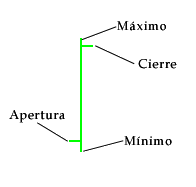
\includegraphics[width=0.4\textwidth]{imagenes/representacion_barra_OHLC.png} 
	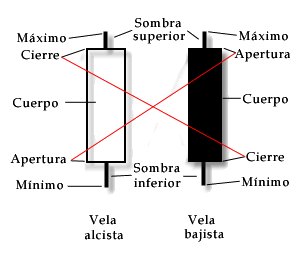
\includegraphics[width=0.5\textwidth]{imagenes/representacion_vela_OHLC.png} 
	\caption{Representación de precios usando barras y velas japonesas. Fuente: \color{blue} \label{ohlc} \href{https://efxto.com/escuela/tipos-de-graficos-de-trading}{Tipos de gráficos de trading y sus características}} 
\end{figure} 

Una vez conocemos los tipos de gráficos de precios de activos financieros, podemos presentar el concepto de temporalidad. La \textbf{temporalidad} o \textbf{marco de tiempo} es la unidad de tiempo o período que elige el trader para ver representado el mercado en el gráfico y estudiarlo. Dependiendo de la temporalidad, el mercado se actualizará cada cierto tiempo, mostrando nuevas velas, barras o puntos, dependiendo del tipo de gráfico que estemos usando. \newline

Como ejemplos de temporalidad podemos ver \textit{M1}, que indica que el gráfico se actualizará con una nueva vela, barra o punto cada minuto; \textit{M5}, que indica un período de actualización de 5 minutos; \textit{H1}, que indica 1 hora; etc. Otras temporalidades son \textit{M15}, \textit{M30}, \textit{H4} (horas), \textit{D1} (días), \textit{W1} (semanas (week)), e incluso actualizaciones mensuales. \newline

A la hora de estudiar los gráficos, la elección del marco de tiempo dependerá de si estamos operando a corto o largo plazo principalmente. Por ejemplo, no tendría mucho sentido estudiar un mercado en M1 si queremos ordenar una operación para una semana vista, ya que no estaremos viendo realmente las tendencias del mercado. \newline



\subsubsection{Precios del mercado: ask y bid}

En esta sección, presento los conceptos de \textit{ask} y \textit{bid}. El \textit{ask} y el \textit{bid} se corresponden con los dos precios que presenta un activo en todo momento. El \textit{bid} es el precio que se ofrece, es decir, el precio que pone el mercado para comprar tus acciones. Por otro lado, el \textit{ask} es el precio que se pide, es decir, el precio de venta del mercado para que el trader compre la acción del activo.  \newline

No importa cuántos vendedores o compradores haya en el mercado en el período a comprar o vender, los precios ask y bid serán el más bajo de todos los ofertantes y el más alto de todos los demandantes, respectivamente. En otras palabras, como traders, venderemos siempre la acción al que más dinero ofrece y compraremos la acción al que más barato la venda. \newline

\subsubsection{Spread}

El \textit{spread} o separación es la diferencia en un momento dado entre los precios \textit{ask} y \textit{bid}. \newline

En el trading, el spread debe de ser pequeño ya que sólo con entrar al mercado estamos perdiendo dinero por esta diferencia de precios. Siempre tendremos que salir a un precio peor con lo que minimizar el spread minimizará las pérdidas. \newline

Este valor es muy alto en ocasiones donde participa muy poca gente en el mercado. En un ejemplo práctico, si sólo hay dos personas en un mercado a un determinado tiempo, y una de ellas vende una acción a 100 \euro y la otra quiere comprar a 60 \euro, el spread es de 40 \euro; probablemente no haya trato. \newline

El spread es una medida de \textit{liquidez}: a menor spread, mayor liquidez. La \textit{liquidez} es en la práctica la facilidad que tienes para comprar o vender al precio que quieres. Esto se ve fácilmente en el anterior ejemplo, donde la liquidez sería baja al tener un spread alto. \newline

En resumen, cuantos más participantes y más activos sean en el mercado, habrá más liquidez ya que el spread será menor; y los precios de compra y venta serán tan parecidos que el spread apenas tendrá impacto en la operativa.

\subsubsection{Volatilidad}

Cuando hay volatilidad en el trading, el precio se acelera. Si estamos usando velas o barras (véase figura \ref{ohlc})), éstas aparecerán más grandes y bruscas en el gráfico.\newline
	
Este fenómeno provoca negociaciones más impulsivas en el gráfico, lo que aumenta el spread. Esto ocurre porque las compras y ventas se realizan de forma más rápida y menos eficientes. \newline

\subsubsection{Cotización}

En el trading, la cotización es el precio de la última operación de un activo o bien el precio al que se vende o compra en el momento actual. En este último caso, la cotización es igual al precio de cierre en el instante. \newline

\subsection{Tipos de análisis de mercados}

Dada esta introducción a lo que es el trading, vemos obvio que lo que buscamos es maximizar los beneficios cuando ordenamos una compra o una venta. \newline

¿Cuándo se debe comprar o vender un activo? Cuando un operador humano piensa en realizar una operación en el mercado, analiza el activo en cuestión siguiendo una serie de criterios basados en distintos tipos de análisis existentes. \newline

\begin{itemize}
	
	\item \textbf{Análisis fundamental}: El análisis fundamental consiste en operar en base a las distintas noticias que ocurren en el mundo diariamente. Estas noticias sirve de fundamento para actuar de una forma u otra en el mercado. 
	\item \textbf{Análisis técnico}: En este tipo de análisis, el operador o trader opera puramente en base al precio: su acción y movimientos. En este caso, no se tienen en cuenta las noticias. Es este el tipo de análisis interesante a la hora de automatizar. Esto ocurre porque en este método entran en juego cálculos matemáticos como medias, medias móviles, zonas de probabilidad estadística, etc. A partir de este análisis surge el trading algorítmico. \\
	Este análisis, aunque se pueda automatizar, no te asegura que el precio vaya en la dirección resultado del análisis. A pesar de esto, si trabajamos con probabilidades y obtenemos probabilidades de ganar superiores al 50\%, obtendremos un sistema que a largo plazo conseguiría grandes beneficios.
	\item \textbf{Análisis de sentimiento}: En este análisis cobran importancia las opiniones de analistas, prensa u observadores de mercados. Este tipo de análisis ocurre mayormente en el \textit{Forex} (mercado de intercambio de divisas).
	\item \textbf{Análisis macroeconómico}: Análisis en el que se tiene en cuenta el comportamiento y desarrollo de la economía de un país. Tiene relación directa con el \textit{Análisis fundamental} ya que las noticias que más afectan a los mercados suelen ser las de corte económico.
	\item \textbf{Análisis cuantitativo}: Este análisis usa lo que se conoce como matemáticas financieras, concepto que deriva de la física y de la estadística.
\end{itemize} 

\subsection{Principales referentes del análisis de mercados}

A lo largo de la historia moderna, economistas, periodistas y demás personas dedicadas a la inversión han desarrollado una serie de estrategias o métodos de análisis de mercados propios. \newline

En concreto, destacamos los cinco principales referentes del análisis de datos de activos financieros: \textit{Charles Henry Dow}, \textit{Richard Demille Wyckoff}, \textit{William Delbert Gann}, \textit{Ralph Nelson Elliott} y \textit{Arthur Alexander Merrill}. \newline

Estas importantes figuras destacaron por sus avances en el ámbito de la economía y todos fueron importantes analistas de mercados. A continuación, cito a cada uno de dichos economistas en orden descendente de antigüedad con sus principales aportaciones a la materia que nos ocupa. \newline

\textit{Charles Dow} (1851-1902) fue cofundador del periódico \textit{Wall Street Journal}. Entre sus avances en destaca la creación del índice de mercado \textit{Promedio Industrial Dow Jones}. \newline

En el caso de \textit{Richard Wyckoff} (1873-1934), se destaca que fue uno de los pioneros en el análisis técnico de mercados de acciones. \newline

El economista \textit{Elliot} (1871-1948) descubrió que el mercado se basaba en principios sociales subyacentes. A principios de los años 20, concluyó que los mercados siguen las leyes de la naturaleza basándose en ratios de \textit{Fibonacci}. Con esto demostró que el comportamiento de los mercados pueden predecirse.  \newline

\textit{Gann} (1878-1955) destacó por sus métodos de análisis de mercados basados en geometría y matemáticas. Se consideraron técnicas innovadoras y se siguen usando a día de hoy. \newline

Por último, el analista \textit{Arthur Alexander Merrill} (1906-2005) destacó por sus aportes en la creación de un sistema de figuras de precios para ser aplicado en el análisis ténico. \newline

Debido al carácter técnico de los análisis propuestos por cada uno de estos autores, y a su respectiva relevancia, en las siguientes secciones se profundiza sobre los análisis o métodos de \textit{Dow} y \textit{Wyckoff}, como posibles candidatos a ser implementados en la aplicación objetivo de este proyecto. \newline

\subsection{Análisis de Charles Henry Dow}

El método de \textit{Dow} se basa directamente en el precio, que refleja el comportamiento humano. Es el indicador más rápido para confirmar una tendencia y se basa en conceptos sencillos pero efectivos. \newline

Este método consistía en un análisis de máximos y mínimos de las fluctuaciones de los mercados financieros, con objetivo de predecir la dirección del mercado. Estos puntos clave son comparados con los máximos y mínimos anteriores. \newline

Dow desarrollo la siguiente teoría, compuesta de 6 principios y llamada la \textit{Teoría de Dow}: \newline

\begin{enumerate}
	
	\item Cualquier acontecimiento externo (fundamento, noticia, etc.) se ve en el gráfico. En otras palabras, los precios son influenciados por dichas situaciones.
	\item Cada mercado financiero tiene tres etapas o tendencias que se repiten:
	\begin{itemize}
		\item \textbf{Primaria}: tendencia a largo plazo, puede durar entre 1 y 3 años.
		\item \textbf{Secundaria}: tendencia a medio plazo, puede durar entre 3 semanas y 3 meses.
		\item \textbf{Terciaria o menor}: tendencia a corto plazo, dura menos de 3 semanas.
	\end{itemize} 
	\item Cada una de las etapas o tendencias primarias presentan 3 fases, que se pueden presentar de dos formas distintas, según si la tendencia es bajista (el precio tiende a bajar) o alcista (el precio tiende a subir):
	\begin{itemize}
		\item \textbf{Tend. prim. alcista}: acumulación $\rightarrow$ tendencia $\rightarrow$ euforia
		\item \textbf{Tend. prim. bajista}: acumulación $\rightarrow$ tendencia $\rightarrow$ pánico	
	\end{itemize} 
	Estas fases se pueden apreciar en la figura \ref{fases_dow}. \newline
	\begin{figure}[h]
		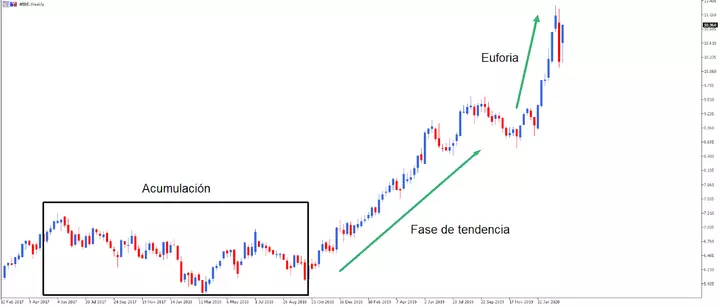
\includegraphics[width=1\textwidth]{imagenes/fases_dow.png} 
		\caption{Fases de acumulación y euforia para tendencia alcista. Fuente: \color{blue} \href{https://admiralmarkets.com/es/education/articles/forex-indicators/teoria-dow}{Teoría de Dow en Análisis Técnico | Dow Theory}} \label{fases_dow}
	\end{figure} \newline
	\item El volumen de negocio confirma la tendencia. El volumen de negocio en trading es la cantidad de un activo en el que se invierte durante un periodo de tiempo. Es un indicador clave de la actividad del mercado y la liquidez.
	\begin{itemize}
		\item Cómo confirma la tendencia alcista: si el precio sube, el volumen aumenta; si el precio baja, el volumen disminuye.
		\item Cómo confirma la tendencia bajista: si el precio sube, el volumen baja; si el precio baja, el volumen aumenta.
	\end{itemize} 
	\item Las tendencias se confirman con los índices \textit{Dow Jones Industrial} y \textit{Dow Jones Transports} (antiguo \textit{Ferrocarril}). Si la tendencia no está confirmada por los índices mencionado tenemos una señal de debilitación de reversión de la tendencia.
	\item La actual tendencia se mantiene vigente hasta que se demuestre el cambio.
	
\end{enumerate} 

En el análisis, Dow considera que en escenarios alcistas se mantiene que tenemos máximos más altos y mínimos más altos. En escenarios bajistas tenemos máximos más bajos y mínimos más bajos. Si no ocurre ni lo primero ni lo segundo, estamos en una situación de mercado lateral o de consolidación. \newline

Dow define en su análisis los siguientes conceptos dentro de los gráficos de precios: \newline

\begin{itemize}
	\item \textbf{Soporte o resistencia:} líneas (o rango) imaginarias en el gráfico de precios que indican zonas. Una vez el precio supera dichas zonas, tenemos una buena posible entrada ya que indica un cambio de tendencia. Indica puntos exactos de entrada al mercado y predice la tendencia.
	\item \textbf{Cascada de mínimos:} la cotización va haciendo mínimos menores. Es una señal de tendencia bajista muy útil para mercados tendenciales con poco retroceso. Se usa un \textit{Stop Lose} más amplio, lo que nos indica un mayor riesgo.
\end{itemize}

Como conclusión, Dow propuso un análisis de mercado para detectar tendencias y períodos de consolidación de los precios. A pesar de que los mercados estén cambiando continuamente, el comportamiento de hoy día en cuanto a dichos conceptos es el mismo que Dow enunció y que recogemos en este apartado.


\subsection{Análisis de Richard Demille Wyckoff} \label{wyckoff}

El aporte de \textit{Wyckoff} fue un enfoque de análisis técnico basado principalmente en la relación entre las fuerzas de la oferta y la demanda. Cuando los grandes operadores quieren comprar o vender, llevan a cabo unos procesos que dejan huella. Dicha huella puede verse en los gráficos de precios de los mercados a través del precio y el volumen. En otras palabras, Wyckoff buscaba ver quién tiene el control del mercado con el objetivo de operar junto a dichos operadores. Para ver estas intenciones de los grandes traders, Wyckoff usaba gráficos de barras y gráficos de Punto y Figura. \newline

\textit{Richard Wyckoff} propuso en sus estudios como analista de mercados financieros, un enfoque en 5 pasos. Este enfoque destaca por su universalidad, ya que puede ser usado en cualquier mercado con suficiente liquidex y en cualquier temporalidad o marco de tiempo. \newline

\begin{enumerate}
	\item Determinar la posición actual y la tendencia futura probable del mercado. Consiste en realizar una evaluación del mercado para ver la tendencia futura y poder tomar decisiones a corto o largo plazo.
	\item Seleccionar acciones acordes con la tendencia. En tendencia alcista, elegir acciones más fuertes que el mercado, es decir, acciones que produzcan mayores aumentos porcentuales que el mercado durante los repuntes y menores disminuciones durante las reacciones. En el caso de tendencia bajista, acciones más débiles que el mercado.
	\item Elegir operaciones con una causa que iguale o exceda su objetivo mínimo. Aquí entra en juego la ley de Wyckoff de causa y efecto. Se eligen acciones que han creado una causa suficiente para su objetivo. Se utilizan proyecciones Punto y Figura.
	\item Elegir acciones disponibles con respecto a la tendencia o fases de acumulación o distribución.
	\item Elegir un buen activo para operar. Un buen activo será aquel que vaya en armonía con el mercado general, lo que proporcionará más probabilidades de éxito.
\end{enumerate}

Uno de sus principales aportes fueron las tres leyes de su método de análisis, el método Wyckoff:\newline

\begin{enumerate}
	\item \textbf{Ley de oferta y demanda.} Si la demanda es mayor que la oferta, el precio sube; si la demanda es menor que la oferta, el precio baja. El trader o analista debe estudiar el equilibrio de oferta y demanda comparando precio y volumen.
	\item \textbf{Ley de causa y efecto.} La causa se mide con el recuento de volumen en un gráfico. El efecto es la distancia que se mueve el precio correspondiente a dicha causa.
	\item \textbf{Ley de esfuerzo y resultado.} Esta ley proporciona una advertencia de un posible cambio de tendencia en un futuro cercano.
\end{enumerate}

En la figura \ref{ciclos_wyckoff} se puede observar cómo la ley de oferta y demanda afecta en la tendencia de un gráfico. En este caso se trata de un boceto de un gráfico de línea. La imagen comienza con una fase de acumulación. Después de esta fase encontramos una clara tendencia alcista seguida de una fase de distribución. Entre la tendencia alcista y la distribución, se vería un patrón indicando una demanda mayor que la oferta. Estos patrones se pueden apreciar estudiando volúmenes, ya que es ahí donde se ve la oferta y demanda. Tras la distribución, la oferta supera a la demanda y la tendencia cambia a bajista.\newline

\begin{figure}[h]
	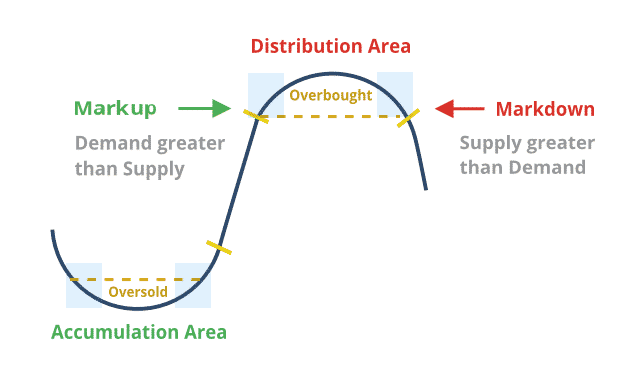
\includegraphics[width=1\textwidth]{imagenes/oferta_demanda_wyckoff.png} 
	\caption{Ciclos del precio de Wyckoff. Fuente: \color{blue} \href{https://www.wyckoffanalytics.com/wyckoff-method-spanish/}{El método Wyckoff}} \label{ciclos_wyckoff}
\end{figure}

Tanto en este análisis como en el de Dow se ha hablado de \textit{acumulación} y de \textit{distribución} pero no se han introducido dichos conceptos. Tanto la fase de acumulación como la de distribución son \textit{rangos de trading}. Los rangos de trading son valores de precios en intervalos concretos en el eje x donde la tendencia que se estaba siguiendo se detiene y hay un equilibrio relativo entre oferta y demanda. La acumulación es el período de equilibrio de oferta y demanda tras venir de tendencia bajista para continuar en alcista. La distribución es la misma zona pero proviniendo de alcista para dar lugar a bajista. \newline

Los rangos de trading y las tendencias serán claves en el análisis de Wyckoff puesto que en su método se estudian estos conceptos y cómo son alterados por la oferta y la demanda. A raíz de estas variables y una serie de decisiones, se ordenará una operación u otra. Concretamente, las decisiones se tomarán en los rangos de trading, puesto que son las principales causas de un cambio de tendencia. \newline

Los 5 enfoques enumerados anteriormente fueron propuestos por Wyckoff de forma teórica. A continuación expongo cómo Wyckoff propuso seguir este enfoque en la práctica. Para ello, Wyckoff describió las fases de acumulación y distribución con una serie de patrones o esquemas que siempre se repetían. Ver estos esquemas nos ayudaría a conocer la tendencia futura y operar.

\subsubsection{Esquemas de acumulación}

A continuación enumero los patrones vistos en una fase de acumulación y que darían lugar a una tendencia alcista. En este caso, si se cumplen los patrones, podríamos entonces ordenar una COMPRA.

\begin{itemize}
	\item Vemos un \textit{PS}, Preliminary Support. Es el patrón que da comienzo a la acumulación. Es cuando la compra de un activo comienza a provocar un soporte en el gráfico. En este momento hay aumentos de volumen y amplitud en los precios, lo que indica que la venta (tendencia bajista) llega a su fin.
	\item Vemos un \textit{SC}, Selling Climax. Es el precio mínimo que se termina formando y que forma el soporte mencionado. Indica que los grandes inversores están comenzando a comprar.
	\item Vemos un \textit{AR}, Automatic Rally. Hay un retroceso en el precio debido a la disminución de la presión de la oferta. Este punto marcaría el techo que serviría como soporte superior del rango de acumulación.
	\item Vemos \textit{STs}, Secondary Tests. El precio fluctúa entre el AR y el SC realizando STs. Podemos encontrar múltiples secondary tests en un mismo rango. Estas fluctuaciones comprueban el equilibrio que hay entre la oferta y demanda en el rango.
	\item Vemos un \textit{SOS}, Sign Of Strength. Avance del precio con rangos más amplios y un mayor volumen.
	\item Vemos un \textit{LPS}, Last Point of Support. Precio mínimo resultado de un retroceso del SOS. Suele coincidir con el techo que había generado el AR, en un menor rango de precios y volumen. Puede haber más de uno aunque se llame last. En la práctica son mínimos más altos desde el AR.
\end{itemize}

En la figura \ref{esquema_acumulacion} se muestran los patrones mencionados en la anterior lista. \newline


\begin{figure}[h]
	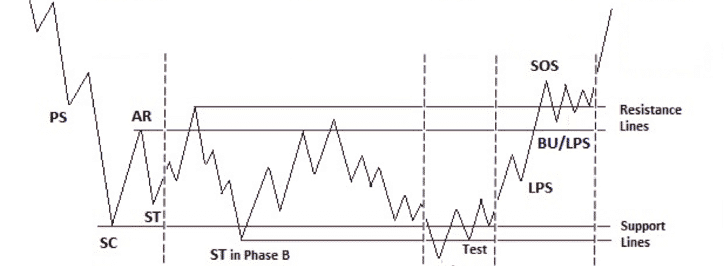
\includegraphics[width=1.1\textwidth]{imagenes/esquema_acumulacion_wyckoff.png} 
	\caption{Esquema de acumulación en el método Wyckoff. Fuente: \color{blue} \href{https://www.wyckoffanalytics.com/wyckoff-method-spanish/}{El método Wyckoff}} \label{esquema_acumulacion}
\end{figure}

\subsubsection{Esquemas de distribución}

En esta sección enumero las pautas seguidas en una fase de distribución y que darían lugar a una tendencia bajista. En este caso, si se cumplen los patrones, podríamos entonces ordenar una VENTA.

\begin{itemize}
	\item Vemos un \textit{PSY}, Preliminary Supply. Es el patrón que da comienzo a la distribución. Es cuando la venta de un activo comienza a provocar un techo en el gráfico. En este momento hay aumentos de volumen y amplitud en los precios, lo que indica que la compra (tendencia alcista) llega a su fin.
	\item Vemos un \textit{BC}, Buying Climax. Es el precio máximo que se termina formando y que forma el techo o resistencia mencionado. Indica que los grandes inversores están comenzando a vender.
	\item Vemos un \textit{AR}, Automatic Reaction. Hay un retroceso en la acción del precio. Este punto marcaría el suelo que serviría como soporte inferior del rango de distribución.
	\item Vemos \textit{STs}, Secondary Tests. Misma definición que en el esquema de acumulación, fluctuaciones entre el AR y el BC, en este caso.
	\item Vemos un \textit{SOW}, Sign Of Weakness. Se sobrepasa el suelo formado por el AR. Avance del precio con rangos más amplios y un mayor volumen.
	\item Vemos un \textit{LPSY}, Last Point of Supply. Precio máximo resultado de un retroceso del SOW. Suele coincidir con el suelo que había generado el AR, en un menor rango de precios y volumen. Vienen a ser máximos más bajos, lo que indica el cambio de tendencia a bajista.
\end{itemize}

En la figura \ref{esquema_distribucion} se muestran los patrones mencionados en la anterior lista. \newline


\begin{figure}[h]
	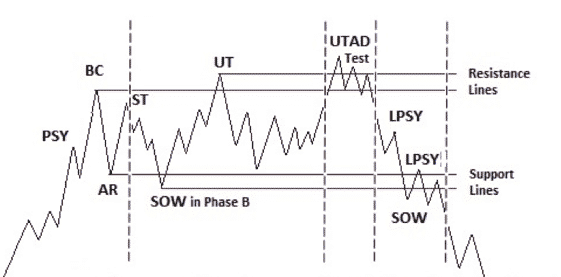
\includegraphics[width=1\textwidth]{imagenes/esquema_distribucion_wyckoff.png} 
	\caption{Esquema de distribución en el método Wyckoff. Fuente: \color{blue} \href{https://www.wyckoffanalytics.com/wyckoff-method-spanish/}{El método Wyckoff}} \label{esquema_distribucion}
\end{figure}


\section{Trading algorítmico}

En pocas palabras, el trading algorítmico es implementar un sistema de trading que opere de forma automática. \newline

El trading algorítmico analiza gráficos de precios de acuerdo a unos criterios preestablecidos, que dependerán del análisis y del propio algoritmo. Cuando el mercado se ajusta a los criterios mencionados, el algoritmo que se ha diseñado para hacer trading ejecutará una acción de compra o venta de manera automática. \newline

Aparte del ahorro de tiempo y esfuerzo, que es la obvia ventaja de usar trading algorítmico, podemos encontrar otros puntos a favor que hacen de las operaciones más eficientes si las comparamos con cómo las haría un operador humano. \newline

\subsection{Ventajas}

\begin{itemize}
	
	\item \textbf{Diversificación}: existe la posibilidad de aplicar un mismo análisis a distintos mercados financieros, aunque puede existir la posibilidad de que en ciertos mercados obtengamos beneficios con una técnica específica que no obtenemos en otro mercado distinto. Esto es más complicado para un operador humano ya que los cambios de acciones de precios en los mercados financieros hacen que un análisis técnico no sea sencillo para un trader acostumbrado a ciertos mercados financieros.
	\item \textbf{Evaluación de técnicas usadas}: debido a que el trading algorítmico automatiza la acción de realizar compras y ventas, podemos evaluar de forma fácil cuándo cierta técnica de análisis es más o menos eficiente en uno u otro mercado. Aquí podemos hablar de distintas horas del día, diferentes temporadas, mercados financieros, etc.
	\item \textbf{Evitar las emociones}: al automatizar un sistema para comprar y vender acciones, el operador humano evita dejarse guiar por las emociones. Esto puede parecer una ventaja simbólica, pero es bastante importante ya que el mercado suele estar sujeto a estadísticas, probabilidades, etc. Si el trader opera suponiendo que cierta vez ocurrirá algo distinto, acaba dejando de lado el análisis puramente técnico. En resumen, evitamos la principal razón por la cual la mayoría de personas que empiezan a dedicarse al trading fracasan, psicología y emociones.
	\item \textbf{Capacidad para desplegar en la nube}: al ser un algoritmo que puede ser desarrollado en un producto software, es posible desplegar o hacer deploy del mismo en un servidor, de manera que el algoritmo desarrollado siempre está conectado al mercado y aplicando reglas para comprar o vender según los criterios mencionados.
	\item \textbf{Precisión y capacidad para realizar compras y ventas de forma simultánea}: el programa sería siempre más preciso que un humano a la hora de realizar entradas y salidas al mercado. Además, puede hacer esto de forma simultánea y operar para distintos mercados financieros a la vez.
	\item \textbf{Posibilidad de aplicar aprendizaje automático}: no sólo podemos centrarnos en desarrollar un algorítmico basado en reglas o análisis del mercado actual sino que también es posible entrenar algoritmos con modelos usando datos históricos de los mercados financieros. Aquí destaca el uso de herramientas de BI y Big Data.
	
\end{itemize}

\subsection{Desventajas}

\begin{itemize}
	
	\item \textbf{Dependencia de noticias}: como se ha mencionado en anteriores apartados de esta memoria, el trading algorítmico surge principalmente del análisis técnico. Aquí destacamos una desventaja del mismo. En el trading algorítmico es muy difícil tener en cuenta noticias que afecten o puedan afectar al comportamiento del mercado en cuestión. Si se decide implementar lógica para estudiar noticias, la complejidad aumenta bastante.
	\item \textbf{Dificultad para detectar la acción del precio}: debido a que el análisis del trading algorítmico es mayoritariamente técnica y basado en cálculos matemáticos, estadística, etc, es complejo detectar la existencia de patrones en el gráfico de precios. Esto sí es más sencillo de realizar por parte de un trader. Entre estos patrones podemos ver soportes, resistencias, líneas de tendencia, niveles, etc. En resumen, es complicado programar una detección de patrones ya que no es algo numérico sino que el operador los identifica a simple vista.
	\item \textbf{Complejidad en la programación}: es realmente complejo programar un algoritmo de trading.
	
\end{itemize}

%
\input{capitulos/03_Planificación}
%
\begin{titlepage}

\chapter{Análisis}



\end{titlepage}

%
\begin{titlepage}

\chapter{Diseño}

% Arquitectura del software, diagramas de clases, diagramas de secuencia

\section{Arquitectura del software}

A continuación muestro un esquema equivalente a la arquitectura general del software.\newline

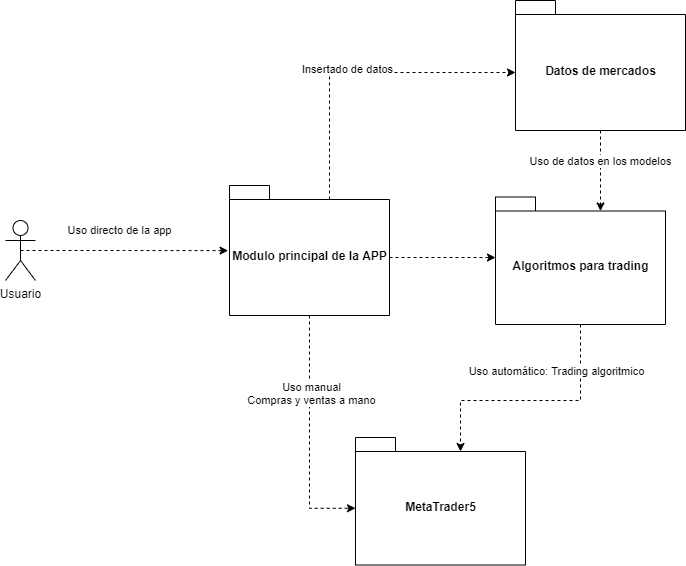
\includegraphics[width=1\textwidth]{imagenes/arquitectura general.png}\\[0.1cm]

Como resumen, en el esquema podemos ver cuál es la idea principal del proyecto. El usuario de la aplicación (véase punto 2.2, segundo implicado) será el que haga un uso directo de la interfaz de la aplicación. A continuación presento cada uno de los módulos con sus funciones y demás utilidades:\newline

\begin{itemize}
	\item \textbf{Módulo principal de la APP}: este módulo se corresponderá con el controlador principal del software. Será usado por el usuario a través de una interfaz escrita en Django y se comunicará con el resto de módulos directamente.
	\item \textbf{Datos de mercados}: este módulo se corresponderá con la base de datos y las operaciones que hagamos con dichos datos (insertado de datos, adaptaciones a cada algoritmo, etc.) Será usado por la interfaz principal de la aplicación y mandará los inputs a los algoritmos.\newline
	\item \textbf{Algoritmos para trading o backend}: se corresponde con el backend o código fuente de la aplicación. Aquí se encontrará cada uno de los algoritmos que usemos para trading algorítmico. Recibe datos de la BBDD y se comunica con el módulo de MetaTrader5 para indicar cada una de las operaciones decididas y obtener información en tiempo real.
	\item \textbf{MetaTrader5}: Módulo externo de la aplicación, se usará para mandar órdenes de operaciones y recibir resultados e información en tiempo real.
\end{itemize}

El software estará escrito en Python, usando Django como Framework para la interfaz web.
% COMPLETAR CON MAS DETALLES DE HERRAMIENTAS

\end{titlepage}
%
\begin{titlepage}

\chapter{Implementación}



\end{titlepage}

%


\chapter{Pruebas}





%


\chapter{Conclusiones}

En este último capítulo destaco las conclusiones que podemos sacar de este trabajo de fin de grado.\newline

Divido esta sección en conclusiones de las pruebas, conclusiones de los objetivos alcanzados y futuras mejoras.\newline


\section{Conclusiones de las pruebas}

En vista de las pruebas obtenidas en el backtesting realizado en el punto anterior, podemos sacar varias conclusiones sobre la eficacia de nuestro algoritmo.\newline

El método de Wyckoff funciona de forma bastante irregular con los mercados financieros de metales y materias primas. Como hemos visto, de las pruebas realizadas en los 4 mercados: XAUUSD, XAGEUR, XBRUSD Y XNGUSD; sólo hemos obtenido un total de 9 operaciones. En otras palabras, al operar en estos mercados, la mayoría de veces mantendríamos el algoritmo funcionando sin que ordene operaciones de compra y venta. Este comportamiento puede deberse a la estabilidad quizás de dichos mercados financieros. Si comparamos estos mercados con los intercambios de divisas, tenemos mercados menos populares y que eso al final, afecta directamente al comportamiento de los precios. \newline

Si un mercado es poco popular entre los operadores, esto supondrá spreads altos, ya que tendremos menos gente que compre al precio que piden los que venden. Spread alto indica menos liquidez. Ver punto 2 de la memoria, contexto teórico del proyecto. \newline

Esto puede ser una justificación de que las operaciones sean malas en dichos mercados. Pero realmente lo que ocurre es que no se ordenan operaciones. \newline

¿A qué puede deberse esto? Bien, la implementación del algoritmo de detección de tendencias, usado en el método de Wyckoff, usaba Bandas de Bollinger. Si volvemos al apartado de implementación, veremos que las Bandas de Bollinger son una medida de volatilidad del precio. Cuando tenemos tendencias bajistas y alcistas, hay más volatilidad en el mercado y es justo con esto con lo que tratamos en el algoritmo. ¿Qué ocurre en el caso de los mercados mencionados, que tienen más spread? Siempre habrá poca volatilidad. Es por esto que nuestro algoritmo tenderá a no encontrar tendencias como lo haría en divisas, donde hay más volatilidad.\newline


Finalmente hablo de los resultados de la ejecución del método de Wyckoff en el mercado de divisas, EURUSD.\newline

En este caso, obtenemos relativamente buenos resultados. En Min15 obtenemos resultados positivos, en H1 también. En la temporalidad de H4, cada 4 horas, hemos obtenido una pérdida; y en D1 hemos obtenido ganancias.\newline

De aquí podemos sacar una conclusión clara, que tiene que ver con la gestión de riesgo. ¿Qué está ocurriendo en Min15 y H1 que no pasa en H4? Estamos aplicando más de una operación, mientras que en H4, sólo realizamos una. Aquí, como he dicho, entra en juego la gestión de riesgo. Cuando definimos el método de Wyckoff, describimos que para ordenar una operacion, el take profit, o valor en el que cerrábamos en ganancias la operación, debería de suponer el doble de ganancias que el stop lose, o valor en el que cerramos con pérdidas. Esto, a efectos teóricos, implica que si hemos realizado dos operaciones; una de ellas beneficiosa y otra con pérdidas; habremos obtenido ganancias en el recuento general.\newline

Por esto, si en H4 se hubiese hecho alguna operación más, tendríamos quizás ganancias, debido a la gestión de riesgo mencionada.\newline

Hablando de nuevo en general de todos los resultados de todos los mercados, no podemos mirar el balance como un número. Este balance debe ser visto como un acierto o una ganancia. ¿Por qué? A la hora de operar en la vida real, los operadores utilizan el lotaje para realizar las inversiones. El lotaje o lote, a efectos prácticos sería el tanto por ciento de activo que compras al invertir. Si compras más lote, tu balance final será el obtenido en estas presuntas situaciones por un multiplicador.\newline

En el caso de la última prueba realizada durante 4 años en la divisa EURUSD en H1 (mencionado al final del capítulo anterior), aunque las ganancias sean pocas, si controlamos el número de lotes, podríamos obtener grandes beneficios. \newline

Como conclusión final, el algoritmo resultante es bueno para operar con EURUSD u otras divisas. Con posibles mejoras, el algoritmo podría ser perfectamente usado por un operador humano en una operativa en tiempo real. En cuanto al resto de mercados financieros, no parece un algoritmo adecuado debido a los problemas antes mencionados. \newline

\section{Objetivos alcanzados}

En la introducción de esta memoria, se hablaba de una serie de objetivos propuestos en el proyecto. En esta sección estudiamos cada uno de ellos y si se ha realizado correctamente o no.\newline

Se han completado todos los objetivos propuestos al inicio del trabajo:

\begin{itemize}
	\item Se ha implementado el sistema de gestión de usuarios
	\item Se ha implementado la conexión con el bróker y plataforma de trading MT5.
	\item Se ha implementado la funcionalidad de ver gráficos en tiempo real del mercado que se quiera visualizar a cualquier marco de tiempo.
	\item Se ha implementado la funcionalidad de ver gráficos de datos antiguos, recogidos de una base de datos previamente guardada por el usuario, de forma automática.
	\item Se ha implementado la estrategia o método de Wyckoff para trading algorítmico.
	\item Se permite a los usuarios realizar operaciones de compra y venta de manera automatizada seleccionando algoritmo.
	\item Se permite a los usuarios realizar backtesting, a modo de prueba de algoritmos.
	\item Se permite a los usuarios ver las operaciones realizadas y balance.
\end{itemize}

También podemos destacar, que el desarrollo del sistema para trading algorítmico cumple con las ventajas expuestas en el apartado de trading algorítmico:

\begin{itemize}
	\item Diversificación: cumplimos con dicha ventaja. A pesar de la menor eficacia en los mercados financieros mencionados, el algoritmo puede ser usado para todos los mercados financieros. Como mencioné en dicha ventaja, existe la posibilidad de que en ciertos mercados obtengamos beneficios con una técnica que no obtenemos con otra.
	\item Evaluación de técnicas: se puede realizar una evaluación numérica de los resultados obtenidos.
	\item Evitamos las emociones.
	\item Podemos desplegar el proyecto en la nube. En este caso, podríamos montar un servidor con Windows que levantase el proyecto y conectarnos a él via internet.
\end{itemize}

\section{Futuras mejoras}

En esta sección propongo posibles futuras mejoras de la aplicación.\newline

Como se ha propuesto en anteriores apartados, mejorar el método de Wyckoff podría ser una posible mejora. En este punto cabría destacar la creación de nuevos análisis de otro tipo de diagramas que Wyckoff expuso en sus enfoques, como bien podría ser el de Punto y Figura. Gracias a estos nuevos análisis, controlaríamos mejor los volúmenes de precios y ofera/demanda, esfuerzo/resultado, etc.\newline

Otra mejora o ampliación sería la inclusión y estudio de nuevos métodos. Esto es sencillo ya que por construcción, la aplicación permite el desarrollo y uso de nuevos algoritmos.\newline

También se podría cambiar o mejorar el sistema de gestión de datos, para poder guardar datos de distintos mercados simultáneamente. Actualmente sólo se permite un mercado con una temporalidad al mismo tiempo. En este punto entraría también la posibilidad de realizar un guardado de dichos datos en la nube.\newline
%
%%\chapter{Conclusiones y Trabajos Futuros}
%
%
%%\nocite{*}
%\bibliography{bibliografia/bibliografia}\addcontentsline{toc}{chapter}{Bibliografía}
%\bibliographystyle{miunsrturl}
%
%\appendix
%\input{apendices/manual_usuario/manual_usuario}
%%\input{apendices/paper/paper}
%\input{glosario/entradas_glosario}
% \addcontentsline{toc}{chapter}{Glosario}
% \printglossary
\chapter*{}
\thispagestyle{empty}

\end{document}
